\documentclass{article}
\usepackage{natbib}

\usepackage{blkarray}% http://ctan.org/pkg/blkarray
\usepackage{amssymb}
\usepackage{amsmath}
\usepackage{array}
\newcommand{\matindex}[1]{{\scriptstyle#1}}% Matrix index

\def\G{{\cal G}}

\def\mmu{\mbox{\boldmath $\mu$}}
\def\th{\mbox{\boldmath $\theta$}}
\def\Sig{\mbox{\boldmath $\Sigma$}}
\def\bbeta{\mbox{\boldmath $\beta$}}

\def\0{\mbox{\boldmath $0$}}
\def\x{\mbox{\boldmath $x$}}
\def\b{\mbox{\boldmath $b$}}
\def\m{\mbox{\boldmath $m$}}
\def\y{\mbox{\boldmath $y$}}
\def\j{\mbox{\boldmath $j$}}
\def\s{\mbox{\boldmath $s$}}
\def\c{\mbox{\boldmath $c$}}
\def\a{\mbox{\boldmath $a$}}
\def\1{\mbox{\boldmath $1$}}
\def\i{\mbox{\boldmath $i$}}

\def\A{\mbox{\boldmath $A$}}
\def\B{\mbox{\boldmath $B$}}
\def\C{\mbox{\boldmath $C$}}
\def\D{\mbox{\boldmath $D$}}
\def\I{\mbox{\boldmath $I$}}
\def\J{\mbox{\boldmath $J$}}
\def\L{\mbox{\boldmath $L$}}
\def\N{\mbox{\boldmath $N$}}
\def\V{\mbox{\boldmath $V$}}
\def\W{\mbox{\boldmath $W$}}
\def\X{\mbox{\boldmath $X$}}

\def\calB{{\mathcal B}}
\def\calL{{\mathcal L}}
\def\calQ{{\mathcal Q}}


\def\tS{\tilde{\S}}
\def\tmu{\tilde{\mu}}
\def\td{\tilde{\d}}

\def\P{\mathbb{P}}
\def\E{\mathbb{E}}
\def\dd{\mathrm{d}}

% Language setting
% Replace `english' with e.g. `spanish' to change the document language
\usepackage[english]{babel}

% Set page size and margins
% Replace `letterpaper' with`a4paper' for UK/EU standard size
\usepackage[letterpaper,top=2cm,bottom=2cm,left=3cm,right=3cm,marginparwidth=1.75cm]{geometry}

% include labels from supplementary
\usepackage{xr}
% --- OVERLEAF XR HELPER CODE ---
\makeatletter
\newcommand*{\addFileDependency}[1]{
  \typeout{(#1)}
  \@addtofilelist{#1}
  \IfFileExists{#1}{}{\typeout{No file #1.}}
}
\makeatother

\newcommand*{\myexternaldocument}[1]{
    \externaldocument{#1}
    \addFileDependency{#1.tex}
    \addFileDependency{#1.aux}
}

\myexternaldocument{supplementary}

% Useful packages
\usepackage{amsmath}
\usepackage{graphicx}
\usepackage{multirow}
\usepackage[colorlinks=true, allcolors=blue]{hyperref}

% references
%\usepackage[round]{natbib} % Allows for Author-Year citations
\bibliographystyle{plainnat} % A style that supports Author-Year

% line number
\usepackage{lineno}

% table rules
\usepackage{booktabs}

% table resize
\usepackage{graphics}

% authors and affiliations
\usepackage{authblk}

% tools
\usepackage{xspace}
\newcommand{\SweepLink}{\texttt{SweepLink}\xspace}
\newcommand{\ApproxWF}{\texttt{ApproxWF}\xspace}
\newcommand{\diplolocus}{\texttt{diplo-locus}\xspace}
\newcommand{\bmws}{\texttt{bmws}\xspace}
\newcommand{\CLUES}{\texttt{CLUES2}\xspace}
\newcommand{\timesweeper}{\texttt{timesweeper}\xspace}

\title{SweepLink: Joint Inference of Demography and Linked~Selection from Time-series Data}
\author[1,2,3]{Ekaterina~Noskova}
\author[1,2]{Madleina~Caduff}
\author[1,2]{Andreas~Fueglistaler}
\author[1]{Anna Parker}
\author[3]{Christoph~Leuenberger}
\author[1,2]{Daniel~Wegmann}

\affil[1]{Department of Biology, University of Fribourg, 1700 Fribourg, Switzerland}
\affil[2]{Swiss Institute of Bioinformatics, 1700 Fribourg, Switzerland }
\affil[3]{Institute of Ecology and Evolution, University of Edinburgh, EH9 3DW Edinburgh, United Kingdom}
\affil[4]{Department of Mathematics, University of Fribourg, 1700 Fribourg, Switzerland}

\begin{document}
\maketitle
\linenumbers

\begin{abstract} % should be below 250 words
Genome-wide time-series data---allele frequency trajectories tracked across multiple sampling times---are among the richest sources of information for inferring selection.
Beyond a beneficial allele's own rise in frequency, such data capture how it drags nearby loci upward via linkage---an effect known as genetic hitchhiking.
Yet most existing tools are single-locus, treating loci independently: they infer site-specific selection coefficients in isolation, then rely on ad hoc window statistics to account for hitchhiking.
Many further require a predefined population size, or scale poorly when jointly inferring demography, and their power is highly sensitive to a significance threshold unknowable in advance.
We present \SweepLink, a two-layer Hidden Markov Model that overcomes these limitations by jointly inferring demography and linked selection genome-wide: a spatial layer captures correlations between neighboring selection coefficients, coupled with a temporal Wright-Fisher diffusion layer.
On simulated data, \SweepLink increases sensitivity to weak and moderate selection while matching existing tools' power to detect strong selection.
By pooling genome-wide evidence, it pushes drift-driven false signals toward neutrality while reinforcing loci with neighbouring support.
This yields confident posteriors that, in practice, remain stable at maximal significance, removing the need for arbitrary thresholds.
We applied \SweepLink to ancient DNA time-series data from the British population, previously analysed with a single-locus tool.
\SweepLink recovers four of the previously reported signals (LCT, SLC45A2, DHCR7, HERC2), and partially recovers the MHC/HLA signal.
It also identifies additional candidate regions---including DPYD, FADS1/2 and OAS1---missed by the prior scan but supported by independent studies.
\end{abstract}


\section{Introduction}

Inference of natural selection is a fundamental task in population genetics.
Selective signals provide critical information about the adaptive processes that have shaped biological populations.
The emergence of ancient DNA (aDNA) has significantly boosted the power of these analyses by providing time-series data.
These temporal data allow for the direct observation of how allele frequencies change over generations.
Under positive selection, beneficial alleles tend to increase in frequency and eventually reach fixation, while negative selection acts to decrease the frequency of deleterious mutations.
By analyzing these allele trajectories, various statistical methods can be employed to estimate the strength and mode of selection.

Inference of selection is intrinsically linked to demography, as failing to account for demographic history is well known to bias selection estimates \citep{jensen2005,nielsen2005,mughal2019}.
To mitigate this bias in case of time-series data, methods generally model genetic drift over time using the Wright-Fisher process within HMM framework.
Recent tools, such as \bmws~\citep{mathieson2022} and \diplolocus~\citep{cheng2025}, successfully scale this framework to genome-wide data by utilizing highly efficient maximum likelihood inference and requiring a predefined effective population size.
Consequently, they provide only point estimates and remain vulnerable to demographic misspecification.
To overcome the dependence on predefined demographic parameters, methods like \ApproxWF~\citep{ferrer2016} employ Bayesian inference to jointly estimate both population size and selection coefficients.
While this joint framework provides a robust solution, its heavy computational burden restricts its application to a small, pre-defined set of candidate loci.

Despite their different strategies for handling demography and computational scalability, all of these methods are fundamentally \textit{single-locus tools}.
By evaluating each site in isolation, they assume that loci evolve independently and thereby ignore the broader genomic context.
This assumption fails to account for the "hitchhiking effect", where selection acting on a causal variant also influences the frequencies of nearby loci.
It has been demonstrated through extensive simulations that ignoring such linked selection leads to significantly biased estimates of selection coefficients \citep{he2020}.
While the method developed in \citep{he2020} can accurately disentangle selection at two linked sites, it does not extend beyond a pair of loci.
One of the first approaches to jointly analyze many linked sites was introduced by \citet{terhorst2015}, which uses a Gaussian process to approximate the multi-locus Wright-Fisher model, capturing linkage-induced correlations between sites through its covariance structure.
However, its quadratic runtime in the number of jointly modeled loci confines inference to small local windows rather than the full genomic landscape.
Another alternative is \CLUES\citep{vaughn2024}, which leverages Ancestral Recombination Graphs (ARGs) to account for linkage, but the computational cost of inferring these genealogies remains a major bottleneck.
Finally, machine learning tools like \timesweeper~\citep{whitehouse2023} scan the genome in windows but require extensive forward-in-time simulations, which are impractical for human populations with large effective population sizes.

To address these limitations, we present \SweepLink, a novel method for the joint inference of demography and linked selection from time-series allele count data.
By incorporating an additional genome-wide layer within its HMM framework, \SweepLink captures correlations between loci, leveraging this linkage to improve selection inference.
Our experiments on simulated data demonstrate that \SweepLink produces a higher sensitivity to weak selection compared to standard single-locus tools.
Moreover, by pooling evidence of selection across the genomic landscape, our method produces more confident posterior probabilities, eliminating the need for arbitrary empirical thresholds to distinguish true from false selective sweeps.
Applying \SweepLink to time-series data from British populations, we recover more known targets of historical adaptation than single-locus method and identify several novel candidate regions.
Although this study focuses on a single-population scenario, the \SweepLink methodology and implementation are developed for multiple populations.


\section{Materials and Methods}

\subsection{Methodological Overview}

\SweepLink is a probabilistic modeling framework designed to jointly infer population sizes, migration rates, and linked selection from time-series allele frequency data.
The method is structured as a two-layer Hidden Markov Model (HMM), illustrated in Figure~\ref{fig:methods:workflow}A.
The first \textbf{spatial layer} models selection coefficients along the genome and accounts for their correlation between adjacent loci through the transition matrix $Q$.
The \textbf{temporal layer} incorporates a diffusion approximation of the Wright-Fisher model to calculate the likelihood of the evolutionary parameters.

\begin{figure}[htbp]
\centering
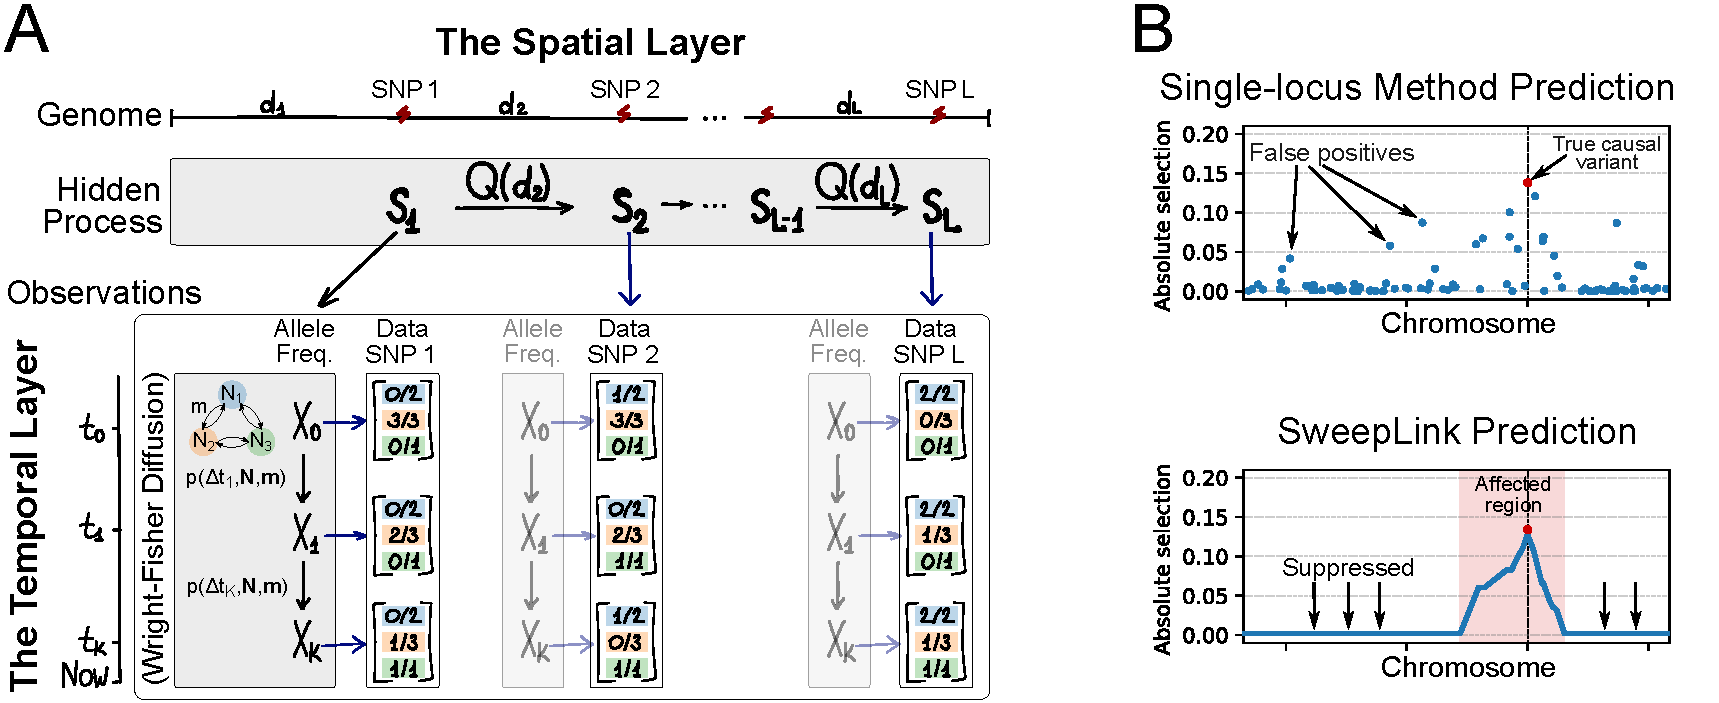
\includegraphics[width=\textwidth]{figures/overview.pdf}
\caption{\textbf{Overview of the \SweepLink Two-Layer HMM architecture.} 
\textbf{(A)} The model framework.
The spatial layer (top, horizontal) models selection coefficients as a hidden Markov process ($ \mathbf{S}_l $) along the genome, with transitions evaluated by distance $ d_l $. 
The temporal layer (bottom, vertical) utilizes a Wright-Fisher diffusion process to calculate the likelihood of observed allele counts. 
These temporal probabilities are jointly parameterized by locus-specific selection ($\mathbf{S}_l$), genome-wide population sizes ($\mathbf{N}$), and migration rates ($\mathbf{m}$). 
\textbf{(B)} Demonstration of selection inference for one population. 
Unlike single-locus methods (top) that are susceptible to noise from genetic drift, \SweepLink (bottom) uses spatial linkage to suppress false-positives and pool true signals into a confident regional peak (red shading).}
\label{fig:methods:workflow}
\end{figure}

The temporal layer itself resembles single-locus methods, such as \ApproxWF or \linebreak \diplolocus, which utilize Wright-Fisher model within the HMM framework.
The spatial layer is the defining feature of \SweepLink that distinguishes it from these approaches.
The ladder-type transition matrix $Q$ defines the hidden process of how selection varies along the genome.
Its parameters constrain adjacent loci to share similar selection coefficients while assuming that the vast majority of the genome evolves neutrally.
This joint HMM framework allows us to use the Metropolis-Hastings Markov Chain Monte Carlo (MCMC) method to infer the parameters of the transition matrix $Q$, the selection coefficients $\mathbf{S}_l$ along the genome, and the demographic parameters $(\mathbf{N}, \mathbf{m})$ directly from the genetic data.

By capturing the correlation of selection coefficients between adjacent loci, \SweepLink models the hitchhiking effect, suppresses isolated false-positive signals caused by genetic drift, and pools signals to form distinct, high-confidence selection peaks (Figure~\ref{fig:methods:workflow}B).

\subsection{Time-Series Data and Underlying Demographic Model}

We first formalize the notation of the input genetic data and the baseline demographic assumptions.
Consider a dataset containing $L$ biallelic variants (SNPs) across the genome.
The physical distance between locus $l$ and locus $l-1$ is denoted as $d_l$.
We have samples at $K + 1$ distinct historical time points defined as $\{t_0 < t_1 < \ldots < t_K\}$.
Genetic data is presented for $P$ populations, and $n_{p, k}$~diploid individuals are sampled for population $p$ at time point $t_k$.
For each locus $l \in \{1, \dots, L\}$ at a given time point $t_k$, the genetic data consists of observed allele counts.
We denote this data as $\mathbf{C}^l(t_k) = \{(c^l_{p,k}, 2n^l_{p,k}),\ p \in \{1, \dots P\}\}$, where $c^l_{p,k}$ refers to the number of observed derived alleles and $2n^l_{p,k}$ is the total number of haploid samples covering that specific locus.
We note that $n^l_{p,k}$ can be less or equal to number of diploid samples $n_{p,k}$ as missing data can occur at individual sites.

We assume these $P$ populations evolve according to structured population model, where each population $p$ maintain a constant effective size of $2N_p$ haploid individuals.
To account for historical admixture, we model continuous migration between all pairs of populations via a constant migration matrix, where $m_{pq}$ denotes the continuous migration rate from population $q$ into population $p$.

\subsection{The Spatial Layer: Genome-wide HMM for Linked Selection}

When a beneficial allele emerges in a population and increases in frequency, the allele trajectories of nearby segregating loci are also affected.
If the causal beneficial allele is in linkage disequilibrium with the derived allele of a neighboring locus, that passenger derived allele will hitchhike and correspondingly increase in frequency.
Conversely, if the beneficial variant is linked to the ancestral allele, the derived allele will decrease in frequency, generating an allele trajectory that mimics the signature of negative selection.
Under the Wright-Fisher model, if a focal allele experiences a selection coefficient $s$, the corresponding alternative allele experiences an inverse selective pressure defined as:
$$s_{inv} = \frac{-s}{1+s}.$$

Recombination breaks down this linkage disequilibrium.
As the physical distance from the causal variant increases, this breakdown of linkage causes the population-level data to show a progressively lower selection coefficient at neighboring loci.
As a result, the selection footprint forms a distinct peak, characterized by high absolute selection coefficients near the causal variant that decline toward neutrality farther away.
Importantly, this pattern depends on the absolute magnitude of selection, as the directional sign ($ s $ or $ s_{inv} $) simply reflects the initial linkage phase of the associated alleles.
The primary objective of the spatial layer is to capture this hitchhiking effect and genetic linkage between loci.

We model the selection coefficient as a hidden Markov process $\mathbf{S}(l)$, where $l$ indexes variants along the genome.
The state $ \mathbf{S}(l) $ is a vector $ (S_1(l), \dots, S_P(l)) $ representing the population-specific selection coefficients.
We assume each $S_p(l)$ evolves as the independent Markov process.
Therefore, we omit the subscript $ p $ for the remainder of this section and describe the process generically for $S(l)$.

To represent selection magnitudes, we define a discrete grid of absolute values $G = \{0, s_1, s_2, \dots, s_M\}$.
Using the inverse selection definition described above, we extend this positive grid to include corresponding negative values:
\begin{equation}\label{eq:sel_grid}
S(l) \in \left\{ - \frac{s_{MAX}}{1+s_{M}}, \dots,  - \frac{s_2}{1+s_2}, - \frac{s_1}{1+s_1}, -0, +0, s_1, s_2, \dots, s_{M}\right\}.
\end{equation}
Two neutral states ($-0$, $+0$) are explicitly retained to maintain balance in the MCMC proposal mechanism.

The state $S(l)$ is decomposed into a direction component $D(l) \in \{+1, -1\}$ and an absolute magnitude component $Z(l) \in G$, as:
$$
S(l) = \begin{cases}
Z(l), & \text{if } D(l) = +1, \\\\
-\frac{Z(l)}{1 + Z(l)}, & \text{if } D(l) = -1.
\end{cases}
$$

Components $D(l)$ and $Z(l)$ are modelled as two independent Markov chains.
The $D(l)$ process has equal probabilities of transitioning between two states, as there is no prior on linkage sign.
The absolute value of selection $Z(l)$ lies within grid $G = \{0, s_1, s_2, \dots, s_{M}\}$.
The transition matrix of this Markov model is inspired by \citet{galimberti2020} and is defined as:
$$Q(d_l) = \exp(d_l \cdot \Lambda),$$
with elements $[Q(d_l)]_{ij}$ denoting the probability of going from state $s_i$ at locus $l-1$ to state $s_j$ at locus $l$ with distance $d_l$ between those loci, either in physical or in recombination space.
The $\Lambda$ is $(M+1)\times(M+1)$ ladder-type generation matrix defined as:
$$
  \Lambda = \kappa \cdot \begin{blockarray}{cccccccccc}
  \matindex{s_0=0} & \matindex{s_1} & \matindex{s_2} & \matindex{s_3} & \ldots & \matindex{s_{M-3}} & \matindex{s_{M-2}} & \matindex{s_{M-1}} & \matindex{s_{M}} &\\
    \begin{block}{(ccccccccc)c}
      -\nu \mu & \nu \mu & 0 & \ldots & 0 & 0 & 0 & 0 & 0 & \matindex{s_0=0} \\
      1 & -1-\mu & \mu & 0 & \ldots & 0 & 0 & 0 & 0 & \matindex{s_1} \\
      0 & 1 & -1-\mu & \mu & \ldots & 0 & 0 & 0 & 0 & \matindex{s_2} \\
      \vdots & \vdots & \vdots & \vdots & \vdots & \vdots & \vdots & \vdots & \vdots & \vdots\\
      0 & 0 & 0 & 0 & \ldots & 1 & -1 - \mu & \mu & 0 & \matindex{s_{M-2}}\\
      0 & 0 & 0 & 0 & \ldots & 0 & 1 & -1 - \mu & \mu & \matindex{s_{M-1}}\\
      0 & 0 & 0 & 0 & \ldots & 0 & 0 & 1 & -1 & \matindex{s_{M}}\\
    \end{block}
  \end{blockarray},
$$
This tridiagonal structure restricts instantaneous transitions to adjacent states on the selection grid, preventing biologically implausible jumps between extreme selection values over short distances.

Transition matrix $Q$ is defined by three parameters: $\kappa$, $\nu$ and $\mu$.
The positive scaling $\kappa$ measures the strength of correlation between loci.
The first row of matrix $\Lambda$ (the attractor) corresponds to the neutrality and has a specific parameter $\nu \in [0,1]$ that defines the probability to leave the neutral state.
The third parameter $\mu \in [0, 1]$ models the rate of moving towards higher value of selection up to $s_M$.

Assuming the absolute magnitude $Z(l)$ and linkage direction $D(l)$ evolve as independent Markov processes, the transition probability for the fully signed state $S(l)$ factors into the product of its components.
As the transition probabilities for linkage direction $ D(l) $ are uniformly equal across the genome, we have $ P(D(l) \mid D(l-1)) = 0.5 $.
Therefore, the joint transition probability between adjacent loci evaluates to:
$$ P(S(l) \mid S(l-1)) = P(D(l) \mid D(l-1)) \cdot P(Z(l) \mid Z(l-1)) = 0.5 \cdot \big[Q(d_l)\big]_{Z(l-1), Z(l)}.$$

Therefore, the probability of a proposed sequence of selection coefficients $ \mathbf{S} = (\mathbf{S}(1), \dots, \mathbf{S}(L)) $ given matrix $Q$ is proportional to:
\begin{equation}\label{eq:spatial_transition}
P(\mathbf{S} \mid Q) \propto P(\mathbf{Z} \mid Q) = P(Z(1)) \prod_{l=2}^L \big[Q(d_l)\big]_{Z(l-1), Z(l)}
\end{equation}
where the probability of the initial state $P(Z(1))$ operates as the stationary distribution of the generator matrix $ \Lambda $.

%Finally, for any proposed state $\mathbf{S}(l)=\mathbf{s}$ at locus $l$, the emission probability $P(\mathbf{C}^l | \mathbf{S}(l) = \mathbf{s})$ is computed by inputting $\mathbf{S}(l)$ into a secondary temporal layer.


\subsection{The Temporal Layer: Hidden Diffusion Model}

The temporal layer produces the emission probabilities $P(\mathbf{C}^l \mid \mathbf{S}(l) = \mathbf{s})$ for the spatial layer at each locus $l$.
The layer is defined by demographic parameters of population sizes $\mathbf{N}$ and migration rates $\mathbf{m}$.
Unlike the locus-specific selection coefficients defined by spatial layer, the demographic parameters are shared globally across all loci.
For simplicity, we will neglect the notation of locus $l$ in this section.

To compute the likelihood of observed allele counts $\mathbf{C}(t)$ at the locus given demographic parameters $(\N, \m, \s)$, we apply an HMM framework in which the hidden states $\mathbf{X}(t)$ are true population allele frequencies evolving as a Wright--Fisher diffusion, and the emissions are binomial samples at each time point:
\begin{equation*}\label{eq:binomial}
\mathcal{B}(\mathbf{c}_k \mid \mathbf{x}_k) :=
\mathbb{P} \big[ \mathbf{C}(t_k) = \mathbf{c}_k \,\big|\, \mathbf{X}(t_k) = \mathbf{x}_k \big] =
\prod_{p=1}^P \binom{2n_{pk}}{c_{pk}}\, x_{pk}^{c_{pk}}\, (1-x_{pk})^{2n_{pk}-c_{pk}}.
\end{equation*}

Briefly, Wright-Fisher diffusion is a continuous-time continuous state Markov process.
Its transition probability density $p(\tau, \mathbf{x}, \mathbf{y})$ --- the probability of moving from frequency $\mathbf{x}$ at time $t$ to frequency $\mathbf{y}$ at time $t+\tau$ --- satisfies the Kolmogorov forward (Fokker-Planck) equation:
\begin{equation}\label{eq:KFE}
\frac{\partial}{\partial \tau} p(\tau, \mathbf{x}, \mathbf{y}) = \frac{1}{2} \sum_{p=1}^P \frac{\partial^2}{\partial y_p^2} \Big[ b_{p}(\mathbf{y})\, p(\tau, \mathbf{x}, \mathbf{y}) \Big] - \sum_{p=1}^P \frac{\partial}{\partial y_p} \Big[ a_p(\mathbf{y})\, p(\tau, \mathbf{x}, \mathbf{y}) \Big],
\end{equation}
where infinitesimal mean (drift) $a_p(\mathbf{y})$ and variance (diffusion) $b_p(\mathbf{y})$ are defined by demographic parameters $\N$, $\m$ and $\s$.
See Supplementary Notes for more details.

Crucially, formulating the temporal layer as a continuous diffusion process allows us to evaluate the likelihood of the time-series data using an efficient forward pass algorithm as in \citet{he2020}.
We define the forward variable $\alpha_k(\tau, \mathbf{y})$ as the joint probability of the hidden frequency state at time $t_k + \tau$ and all observed data up to time $t_k$:
$$
\alpha_k(\tau, \mathbf{y}) = \mathbb{P}\big( \mathbf{X}(t_k+\tau) = \mathbf{y},\, \mathbf{C}(t_0) = \mathbf{c}_0, \ldots, \mathbf{C}(t_k) = \mathbf{c}_k \big)
$$
It can be shown that the recursive update of the forward variable:
$$
\alpha_k(0, \mathbf{y}) = \mathcal{B}(\mathbf{c}_k \mid \mathbf{y}) \int_{(0,1)^P} \alpha_{k-1}(\Delta t_{k-1}, \mathbf{x}) \, p(\tau, \mathbf{x}, \mathbf{y}) \, d\mathbf{x}
$$
can be replaced by the the forward Kolmogorov equation~\ref{eq:KFE}:
\begin{align}\label{eq:KFE_alpha}
\frac{\partial}{\partial \tau} \alpha_k(\tau, \mathbf{y}) &=  \frac{1}{2} \sum_{p=1}^P \frac{\partial^2}{\partial y_p^2} \Big[ b_{p}(\mathbf{y})\, \alpha_k(\tau, \mathbf{y}) \Big] - \sum_{p=1}^P \frac{\partial}{\partial y_p} \Big[ a_p(\mathbf{y})\, \alpha_k(\tau, \mathbf{y}) \Big] \\
\intertext{subject to the initial condition:}
\label{eq:KFE_alpha_init}
\alpha_k(0, \mathbf{y}) &= \alpha_{k-1}(\Delta t_{k-1}, \mathbf{y}) \, \mathcal{B}(\mathbf{c}_k \mid \mathbf{y})
\end{align}

Consequently, we can iteratively evaluate the forward pass from $k = 0$ to $K$ by numerically solving this partial differential equation~\ref{eq:KFE_alpha} across sequential time intervals.
To establish the base case for this induction at the first sampling time point ($k = 0$), the recursion is initialized using the prior density $\alpha(\mathbf{y})$, such that $ \alpha_0(0, \mathbf{y}) = \alpha(\mathbf{y}) \mathcal{B}(\mathbf{c}_0 \mid \mathbf{y}) $.
For all subsequent time points, the final solution from the preceding interval, $ \alpha_{k-1}(\Delta t_{k-1}, \mathbf{y}) $, is substituted into Equation~\ref{eq:KFE_alpha_init} to continuously initialize the next numerical integration.

Once the forward pass reaches the final sampling time point $t_K$, the total likelihood of the model is obtained by integrating the final forward variable $\alpha_K$:
\begin{equation}\label{eq:spatial_emission}
\mathbb{P}(C(t_0)=c_0, \dots, C(t_K) = c_K \mid \mathbf{S}, \mathbf{N}, \mathbf{m}) = \int_{(0, 1)^P} \alpha_K(0, \mathbf{y})\, d\mathbf{y}.
\end{equation}
Because evaluating these multidimensional partial differential equations analytically is broadly intractable, we discretize the state space and solve the forward operator numerically using the Chang-Cooper numerical scheme~\cite{chang1970,pareschi2018} and alternating direction method~\cite{press2007} (for more details see Supplementary Note X).
We implement several types of grid~\citep{gutenkunst2009,cheng2025, malaspinas2012} for the relative allele frequency space in Hidden Diffusion and empirically test them.
Chebyshev grid provides the most robust performance (see Supplementary Note X and Figure SX).

\subsection{Bayesian Inference and Parameter Estimation}

To infer the evolutionary history from the time-series data, we employ a Bayesian framework to estimate the joint posterior distribution of the model parameters.
We first summarize the complete set of parameters estimated within the \SweepLink model.
The spatial layer introduces $\mathbf{S} = \{\mathbf{S}(1), \mathbf{S}(2), \dots, \mathbf{S}(L)\}$ as the hidden sequence of locus-specific selection states along the genome, alongside the parameters $\boldsymbol{\kappa}, \boldsymbol{\nu}, \boldsymbol{\mu}$ that define the transition matrix $Q$.
The parameter space is subsequently completed by the global demographic variables $\mathbf{N}$ and $\mathbf{m}$ derived from the temporal layer.
Given the observed allele count data $\mathbf{C}$, the posterior distribution for the parameter set $\boldsymbol{\theta} = (\mathbf{S}, \boldsymbol{\kappa}, \boldsymbol{\nu}, \boldsymbol{\mu}, \mathbf{N}, \mathbf{m})$ is proportional to:
$$
P(\boldsymbol{\theta} \mid \mathbf{C}) \propto P(\mathbf{C} \mid \boldsymbol{\theta}) \cdot P(\boldsymbol{\theta}) = \left[ \prod_{l=1}^L P(\mathbf{C}(l) \mid \mathbf{S}(l), \mathbf{N}, \mathbf{m})\right] \cdot P(\mathbf{S} \mid Q_{\boldsymbol{\kappa}, \boldsymbol{\nu}, \boldsymbol{\mu}}) \cdot P(\boldsymbol{\kappa}, \boldsymbol{\nu}, \boldsymbol{\mu}, \N, \m).
$$
Here, the locus-specific emission probability $P(\mathbf{C}(l) \mid \mathbf{S}(l), \mathbf{N}, \mathbf{m})$ is defined by Equation~\ref{eq:spatial_emission}, the probability of drawn selection coefficients $P(\mathbf{S} \mid Q_{\boldsymbol{\kappa}, \boldsymbol{\nu}, \boldsymbol{\mu}})$ is defined by Equation~\ref{eq:spatial_transition}, and $P(\boldsymbol{\kappa}, \boldsymbol{\nu}, \boldsymbol{\mu}, \N, \m)$ evaluates as the combined product of the independent parameter priors.

We utilize a Markov chain Monte Carlo (MCMC) algorithm to draw representative samples directly from this posterior distribution.
Specifically, we execute a Metropolis-Hastings sampling\linebreak scheme~\citep{metropolis1953,hastings1970} that iteratively proposes new parameter values and hidden states, accepting or rejecting them based on the evaluated ratios of this unnormalized posterior distribution.

\bigskip

To translate the resulting MCMC trace into quantitative evidence for selection at any given locus, we approximate the marginal posterior probabilities directly from the parameter samples. 
Let $W$ be the total number of MCMC samples. 
For any specific selection coefficient $s$ on the fully signed discrete grid, its estimated posterior probability is calculated as its sample frequency, utilizing a smoothing correction defined as $ X_s / (W + 1) $, where $ X_s $ is the number of MCMC samples yielding state $ s $.
We then calculate the posterior probability $P(s > 0)$ of positive selection, and probability $P(s < 0)$ of negative selection by summing these estimates across all strictly positive and strictly negative states on the grid.
Finally, to summarize the model's overall confidence in directional selection, we define our primary classification score as:
\begin{equation}\label{eq:final_posterior}
    P = \max(P(s > 0), P(s < 0)).
\end{equation}
This value serves as \SweepLink’s primary statistic to distinguish between neutral variants and selective sweeps.

\subsection{Implementation}

The proposed model and the Bayesian inference scheme are implemented in an easy-to-use C++ program \SweepLink, available at \url{https://bitbucket.org/wegmannlab/sweeplink/}.
We provide complementary Python 3 scripts to process VCF files into \SweepLink input and to post-process \SweepLink output, including plotting of the results.
Detailed documentation and a tutorial can be found at \url{https://sweeplink.readthedocs.io}.

\subsection{Benchmarking Against Competitor Single-Locus Tools}

\paragraph{Simulated Benchmark Dataset.}
To perform a benchmark analysis of \SweepLink, we generate a simulated dataset using the forward-in-time simulator SLiM v4~\citep{haller2023}.
We generate ten short chromosomes, each with a length of 0.1~Mb.
Half of chromosomes contain only neutral mutations.
The remaining five chromosomes have a hard selective sweep introduced at the middle position, with a selection coefficient equal to $0.01$, $0.02$, $0.03$, $0.04$, or $0.05$, respectively.
Population parameters are chosen to resemble realistic human populations: population size was set to $N=10{,}000$ individuals~\citep{takahata1993}, mutation rate to $\mu_{aA} = 10^{-8}$ per site per generation~\citep{kong2012}, and recombination rate to $r=10^{-8}$~per site per generation~\citep{kong2002}.

Sampling is performed once the selected allele reaches a frequency of 30\%.
Genetic data are sampled at $K=11$ consecutive time points, with $\Delta t=16$ generations between each, thereby spanning 160 generations.
This sampling regime reflects the real human data analyzed in this study, which includes samples dating approximately 4,000 years before present.
At each time point, genetic data for $n=25$ diploid individuals were sampled.
To generate the robust benchmark dataset, this entire simulation setup was replicated 100 independent times, yielding a total dataset of exactly 500 independent selective sweeps (100 for each selection coefficient) against a background of over 100,000 strictly neutral variants unlinked to the targets of selection.
We filtered the dataset to retain only sites where the derived allele segregates at a minimum of two sampled time points, removing on average ~21\% of variants.
As shown in the Supplementary Material, this filter does not affect inference accuracy but reduces runtime.

\paragraph{Detection Power Evaluation.}
We evaluate the performance of \SweepLink against three established single-locus tools: \ApproxWF~\citep{ferrer2016}, \diplolocus~\citep{cheng2025}, and \bmws~\citep{mathieson2022}.
To ensure a fair comparison, the true simulated effective population size ($ N=10{,}000 $) is explicitly provided as a fixed, known value to all methods.
\SweepLink is launched with 50 grid points for the numerical scheme of the diffusion equation and a discrete selection grid of 13 states for positive selection magnitudes from $s=0.0$ to $0.06$ with a step size of $0.005$.
This grid is extended in \SweepLink to include corresponding negative selection values following Equation~\ref{eq:sel_grid}.
The same complete grid is used for the maximum-likelihood approach in \diplolocus, which calculates the likelihood values across the grid and then interpolates them to find the off-grid maximum.
We run \ApproxWF and \bmws with default parameters as recommended in their documentation.
If not specified otherwise, MCMC in \ApproxWF and \SweepLink is run for 100,000 samples.

First, we evaluate and compare the power of each tool to detect selection.
We frame the problem as a binary classification task: how well each tool distinguish neutral loci from those under directional selection, regardless of the estimated selection coefficient.
Because random genetic drift generates background noise and can mimic trajectories similar to the selection process, raw quantitative estimates of selection cannot be taken as definitive proof of an actual sweep.
Instead, the raw outputs of the selection from tools must be further processed to produce scores that quantify the evidence for selection.
Once these scores are obtained, a formal discovery threshold is applied to binarily classify each locus as either strictly neutral or under directional selection.

We extract specific metrics from each tool as scores for this classification task.
For \diplolocus, we directly utilize the $p$-value derived from its likelihood ratio test~\citep{cheng2025}. 
For \bmws, we follow the statistical framework described in its original publication~\citet{mathieson2022}.
We aggregate single-locus selection estimations within sliding windows of 20 SNPs, approximate a gamma distribution, and derive a $p$-value by testing whether the window estimation deviates from this distribution.
Finally, both \SweepLink and \ApproxWF utilize MCMC-based Bayesian inference to yield posterior distributions for the selection coefficient. 
In its original implementation, \ApproxWF consider loci to be under selection if the 95\% credible interval of the posterior distribution excludes zero~\citep{ferrer2016}. 
However, to ensure a fair comparison, we use the same score from Equation~\ref{eq:final_posterior} as in \SweepLink, defined as $P = \max(P(s > 0), P(s < 0))$.
We note that this metric for \ApproxWF and \SweepLink has an upper bound defined by the number $W$ of MCMC samples: $P \leq \frac{W}{W+1}$.

To translate these continuous statistical scores into a binary classification, a formal discovery threshold must be applied. 
For example, a researcher might classify a locus as selected only if it achieves a $p$-value $< 10^{-7}$ or a posterior probability $> 0.99$, treating all loci that fail to meet this threshold as neutral.
An optimal threshold must maximize true positives (the correct identification of actual selective sweeps) while minimizing both false positives (the incorrect flagging of neutral loci) and false negatives (missed sweeps).
To identify the optimal threshold and best performance for each tool, we evaluate the global classification accuracy across a continuous spectrum of all possible discovery thresholds. 

As a representative metric for detection accuracy, we calculate the Matthews correlation coefficient~(MCC)~\citep{matthews1975} for each threshold.
The MCC is defined as:
$$
\text{MCC} = \frac{TP \times TN - FP \times FN}{\sqrt{(TP + FP)(TP + FN)(TN + FP)(TN + FN)}}
$$
where $TP$ (True Positives) represents the number of correctly identified loci under selection, $TN$ (True Negatives) represents the number of correctly identified neutral loci, $FP$ (False Positives) is the number of neutral loci wrongly classified as selected, and $ FN $ (False Negatives) is the number of selected loci wrongly classified as neutral.
The MCC yields a value between $-1$ and $1$, where $1$ indicates perfect classification, $0$ indicates performance no better than random guessing, and $-1$ indicates total disagreement between predictions and the true labels. 
We specifically chose the MCC as an improvement over the classic $F_1$ score, which can be highly misleading when applied to datasets with imbalanced classes~\citep{chicco2020}, such as our simulated dataset containing roughly 80,000 neutral variants but only 500 selective sweeps.
Therefore, by evaluating MCC accross a spectrum of possible thresholds, we discover the optimal threshold as the threshold yielding best MCC score.
We compare tools by their best MCC scores and investigae how threshold selection impacts their power to detect selection.

\paragraph{Correlated False-Positives and Window-based Comparison.}
When calculating MCC scores for given dataset, \SweepLink provides the best detection power among tools (Table~\ref{tab:no_window}), but the number of false positives is also the highest (e.g. 0.05\% vs 0.01\% for \ApproxWF).
Because \SweepLink pools evidence across linked loci, drift that happens to mimic selection at several linked sites can trigger correlated false positives across an entire linked block, inflating its false-positive rate under locus-level MCC scoring.
To avoid this bias, we evaluate detection performance over $k=21$ alternating, non-adjacent windows per chromosome ($\sim$9{,}500\,bp apart) rather than individual loci.
A window is called positive if any locus within it is significant given current threshold.
The middle window of a selected chromosome --- the one containing the true sweep --- is scored as a true positive (TP) if positive and a false negative (FN) otherwise.
Every other window, on any neutral chromosome, is scored as a false positive (FP) if positive and a true negative (TN) otherwise.
This window-based comparison collapses correlated false positives from a linked block into a single call, ensuring a fair comparison between tools.

\paragraph{Selection Coefficient Accuracy.}
We further compare the detection sensitivity and estimation accuracy of each tool across strictly neutral sites ($s=0.0$) and five distinct categories of positive selection ($s \in \{0.01, 0.02, 0.03, 0.04, 0.05\}$).
Thresholds are chosen so that all methods are aligned to an identical window-based False Positive Rate (FPR) of 0.3\%, corresponding to the baseline error rate achieved by \SweepLink at its optimal threshold.
For each selection coefficient, we report the detection rate as the rate at which each tool correctly predicts the selection at the corresponding loci regardless of the estimated value. 
To compare accuracy for correctly detected selection sweeps, we compare the mean and variance of the estimated selection coefficients ($\hat{s}$) at the true sweep locus.
To avoid biasing this comparison toward zero, we exclude sweeps misclassified as neutral (false negatives) from this analysis.
Additionally, we compare the dispersion of $\hat{s}$ for neutral variants
misclassified as sweeps (false positives), taken from the locus that triggered the
window's significance.

\subsection{\SweepLink Robustness and Parameter Sensitivity}

In a separate experimental setup, we evaluated the robustness and parameter sensitivity of the \SweepLink framework under diverse evolutionary and sampling scenarios.
We used data simulated by SLiM with a configuration described in previous section as a default configuration.
The only difference is that three selection coefficients are analysed instead of five: weak $s=0.01$, moderate $s=0.01$ and strong $s=0.05$.
Therefore, six chromosomes of 0.1 Mbp are simulated instead of ten as in the previous setup.
This default configuration serves as baseline for subsequent experiments.
To assess the impact of individual parameters on the accuracy of \texttt{SweepLink}, we varied one characteristic at a time---for example, sample size, sequence length or recombination rate---while keeping all other parameters constant at their default values.
This approach enables us to quantify how each parameter influences the accuracy of inference.

In summary, we test \texttt{SweepLink} across the following characteristics: 1) sample size, 2) sequence length, 3) number of time points, 4) binning size, 5) starting allele frequency of the selective sweep, 6) recombination rate, and 7) grid size in the numerical scheme for the diffusion equation.
See Supplementary Materials for further details on specific values that are tested.
For each experimental setup, simulation and inference are repeated across 100 independent runs.
\SweepLink performance is measured by the power to detect selection---true positive rate on the optimal threshold---and by relative error of selection coefficient estimation.
Both metrics are evaluated for each selection coefficient ($0.01$, $0.02$, $0.05$) separately to validate the performance on weak, moderate and strong selection.
We also additionally check the stability of detection power of \SweepLink using MCC metrics evaluated on the spectrum of thresholds as described in the previous section.

\subsection{Empirical Data}
We apply \SweepLink on the British ancient-DNA time series dataset that was analysed previously using \bmws in~\citet{mathieson2022} and constructed from several resources~\citep[version 44.3]{mallick2024}\citep{martiniano2016,schiffels2016,olalde2018,brace2019,margaryan2020,patterson2022,1000G2015}.
Dataset contains 627 pseudo-haploid samples genotyped on 1240k SNPs: 535 ancient samples and 92 present-day samples.

Sample dates are converted to generations assuming 29 years per generation and binned into 5-generation intervals, giving 26 timepoints spanning $0{-}150$ generations before present ($0{-}4{,}350$ years).
Sampling density is uneven across this range (Figure~\ref{fig:british_data_sampling}): the oldest sample dates to $4{,}480$ BP and the youngest ancient sample to 930 BP, nearly half of all ancient chromosomes fall within ${\sim2{,}000-2{,}300}$ years BP.

\begin{figure}[btp]
    \label{fig:british_data_sampling}
    \centering
    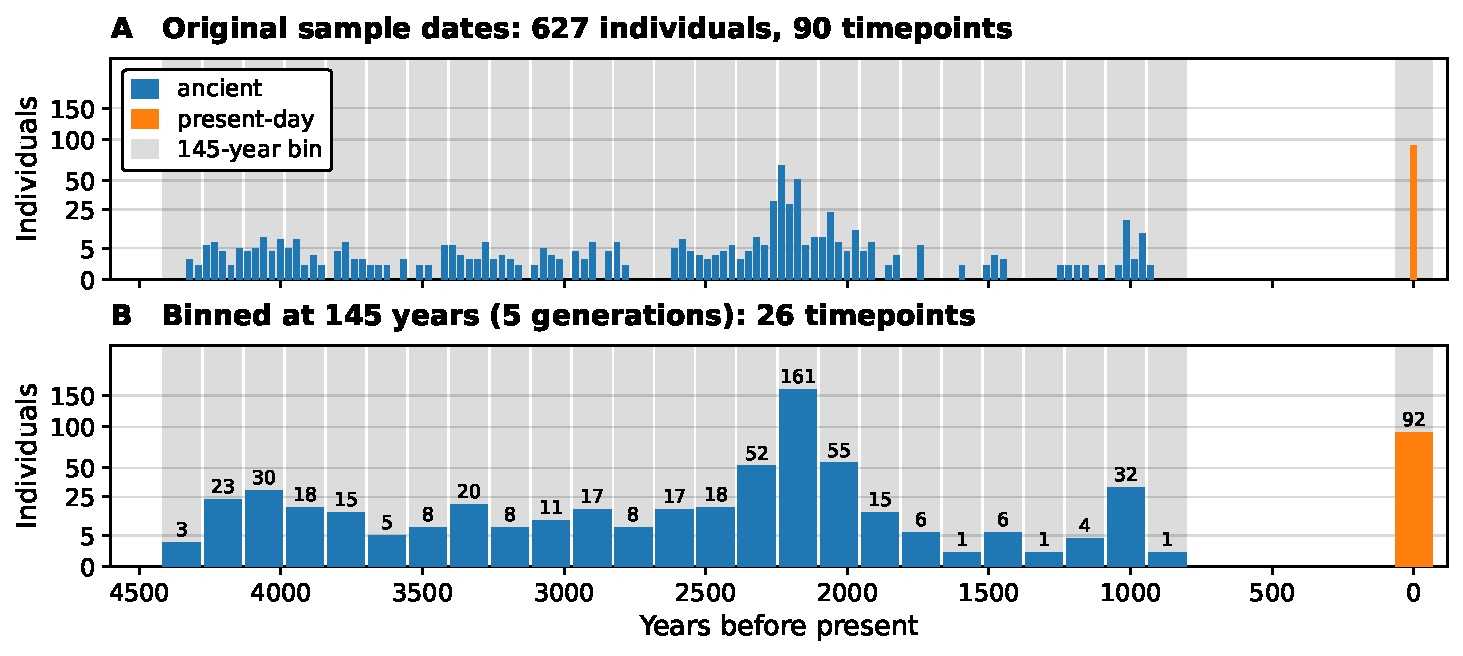
\includegraphics[width=\textwidth]{figures/fig_sampling.pdf}
    \caption{Temporal sampling of the British ancient-DNA dataset, before and after binning.
    \textbf{A}~The dataset assembled from~\citet{mathieson2022} contains 627 pseudo-haploid individuals at 90 distinct timepoints. 
    \textbf{B}~After binning by 5 generations of 29 years, 26 timepoints of 145 years remain.
    Shaded bands mark the bins and bars are labelled with the number of individuals they contain.
    }
\end{figure}

Starting from $1{,}150{,}639$ autosomal SNPs, we remove 151 sites with no called genotypes and $144{,}019$ sites monomorphic across the dataset.
Then we apply filters for missing genotypes to remove number of sites with low-quality data.
We remove 437 sites at which more than 45\% of the present-day panel is uncalled and $149{,}822$ sites at which more than 80\% of the ancient samples are uncalled.
Finally, to make our inference faster without losing valuable data, we remove $39{,}296$ sites whose derived allele segregated at fewer than two timepoints.
In a separate experiment, we confirmed that such filtering does not affect the estimation accuracy of \SweepLink (see Section~\ref{}). %TODO
We do not use MAF filtering as in the original study~\citep{mathieson2022} to avoid bias in population size estimation.
This leaves $816{,}914$ SNPs genome-wide (71\% of the starting set).

We split the dataset by chromosome and used \SweepLink to infer a selection coefficient at every locus together with an effective population size for each chromosome.
A locus is called as potentially causal for selection when all 100,000 MCMC iterations agree on the sign of selection coefficient.
At this chain length the criterion corresponds to a posterior probability of at least 0.99999, and in our simulations this maximum-stringency threshold gave \SweepLink its best detection performance (Section~\ref{sec:threshold}).
At such loci we report the posterior mean of $s$ over the signed grid.

Because \SweepLink models linkage between neighbouring loci through a hidden Markov chain along the genome, evidence for selection is shared within a region and a detected locus rarely stands alone.
We therefore report regions together with an individual loci.
We define a region as a maximal run of consecutive SNPs at which the posterior probability of neutrality is below 0.5, and regard a region as affected by selection when it contains at least one locus that was detected as potentially causal variant for selection using criterion above.

Loci identified as potentially causal variants for selection are carried through a common annotation pipeline.
Associations were retrieved from OpenGWAS~\citep{elsworth2020opengwas}, which aggregates the NHGRI-EBI GWAS Catalog~\citep{buniello2019}, UK Biobank~\citep{bycroft2018} analyses from the MRC-IEU~\citep{elsworth2019ukb} and Neale laboratory pipelines~\citep{nealelab2018ukb}, and molecular-trait scans including eQTLGen whole-blood \emph{cis}-eQTLs~\citep{vosa2021}.
We queried every batch except FinnGen and BioBank Japan, whose populations differ too much from the British sample in linkage structure.
Where associations are found we test whether the selection signal and the GWAS signal are consistent with a shared causal variant by approximate Bayes factor colocalisation, reporting the posterior probability of a common causal variant (PP$_4$)~\citep{giambartolomei2014}.
We apply colocalisation analysis using a 1~Mb window centred on the target variant ($\pm$500~kb) and the prior probabilities $p_1 = p_2 = 10^{-4}$ and $p_{12} = 10^{-5}$.

Detected variants are additionally annotated with the Ensembl Variant Effect Predictor \citep{mclaren2016} to establish their functional consequence and their overlap with annotated regulatory features.
For each region identified to be affected by selection we plot the inferred selection signal alongside the 1000 Genomes Phase~3 recombination map~\citep{1000G2015,howie2009}, to establish whether peaks coincided with regions of reduced recombination.
For the lactase LCT region on chromosome 2 we additionally show the surrounding linkage disequilibrium block using the European block boundaries identified by LDetect~\citet{berisa2015}.

\section{Results}

\subsection{Strong posterior support eliminates the need for threshold tuning}
\label{sec:threshold}

The result window-based MCC values across the discovery thresholds for each tool are presented in Figure~\ref{fig:results:mcc_plot}.
\SweepLink shows the highest peak performance (MCC = 0.87), ahead of \diplolocus (0.8), \ApproxWF (0.85) and \bmws (0.77).
Each tool reaches its optimum at a threshold specific to its own score scale, but they differ in the shape of their threshold dependence and in how wide a range of thresholds sustains near-optimal performance.
The latter is important, because the optimal threshold is unknown in real empirical applications, and researchers are forced to rely on standard conservative heuristics, such as a Bonferroni-corrected significance level~\citep{cheng2025}. 
The narrower the optimal plateau, the more that choice costs.
The region retaining performance within 0.01 MCC of the peak spans 1.6 orders of magnitude for \SweepLink and 1.2 for \diplolocus, but only 0.7 for \ApproxWF and 0.2 for \bmws, after which performance declines steadily.
At the high stringencies typically required for genome-wide scans
($\sim 10^{-7}$), \diplolocus falls from its optimum of 0.86 to 0.78, and \bmws from 0.77 to 0.07.
\ApproxWF reports a posterior probability rather than a $p$-value, so it is not subject to the same correction, but it is no less threshold-dependent: its optimum lies at a very lenient $1-P \approx 0.3$, and demanding higher confidence costs it 0.09 MCC by $1-P = 10^{-4}$.

\begin{figure}[t]
\centering
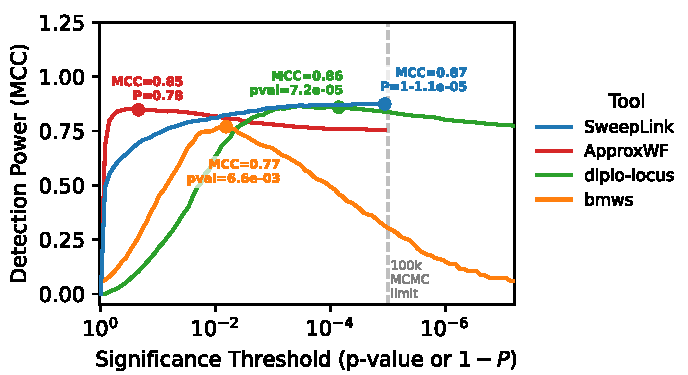
\includegraphics[width=0.6\textwidth]{figures/MCC/comparison_power_plot_no_1M.pdf}
\caption{\textbf{Power to detect selective sweeps across discovery thresholds.}
The x-axis displays native $p$-values (\diplolocus, \bmws) or $1-P$ (\SweepLink, \ApproxWF), where $P = \max(P(s>0), P(s<0))$.
Markers denote peak MCC.
Unlike standard methods, \SweepLink receives peak accuracy on maximum possible threshold ($P=1.0 - 10^{-5}$) in its default run.
The extended run of \SweepLink \texttt{(1M)} for 1 million samples demonstrate the best MCC score and shows stable plateaux on for the range of the stringent thresholds ($P > 1 - 10^{-4}$).
}
\label{fig:results:mcc_plot}
\end{figure}

\SweepLink also reports a posterior probability as \ApproxWF, but its optimum lies at the opposite end of the scale.
It achieves the widest plateau of any tool tested and remains stable throughout the entire high-confidence domain ($1-P < 10^{-4}$): 0.87 at $10^{-4}$ and 0.88 at $10^{-5}$.
Crucially, \SweepLink reaches its optimal performance at the theoretical limit of maximum confidence ($1-P \sim 10^{-5}$), which is set by the length of the MCMC chain: a posterior probability estimated from $W$ samples cannot be resolved beyond $1/(1+W)$.
Demanding the highest confidence the method can express is therefore also the best-performing choice, so no threshold tuning is required and the problem of an unknown optimum does not arise.
The measured plateau width is consequently a lower bound rather than a property of the estimator: running an extended chain of 1,000,000 samples reproduces the same plateau and extends it by a further order of magnitude (Supplementary Figure~\ref{fig:supp:mcc_1M}), confirming that the limit reflects the resolution of the estimator rather than its discriminative power.

As detailed in subsequent experiments, this robust plateau of \SweepLink with peak at maximum threshold is consistently maintained across diverse evolutionary scenarios, bounded only by the fundamental limits of genetic linkage (Figure~\ref*{fig:supp:power_analysis}).
Specifically, under extreme recombination rates ($r \ge 10^{-6}$ relative to a mutation rate of $10^{-8}$), the physical footprint of a sweep becomes too narrow to provide a meaningful regional context.
In these isolated cases, the performance of \SweepLink converges toward single-locus behaviour, exchanging its high-confidence plateau for a distinct performance peak at more lenient thresholds (Figure~\ref*{fig:supp:power_analysis:rec_rate}).
% TODO: below to discussion?
However, because such extreme recombination regimes represent only a small fraction of typical genomes, \SweepLink remains uniquely suited for general ``out-of-the-box'' empirical scans.
Researchers can simply demand maximum statistical certainty to achieve optimal detection power, without sacrificing true positive discoveries or risking an inflated false-positive rate.


\subsection{Sweep Detection Sensitivity and Estimation Accuracy}

Result detection rates for five distinct categories of positive selection ($s \in \{0.01, 0.02, 0.03, 0.04, 0.05\}$) are presented in Figure~\ref{fig:results:tools_comparison}A.
While all methods successfully identified strong selective sweeps ($s \ge 0.03$), \SweepLink demonstrated vastly superior sensitivity for weak selection.
For instance, \SweepLink successfully recovered 17\% of the weakest sweeps ($s = 0.01$), whereas single-locus methods (\diplolocus, \ApproxWF) detected only a fraction ($9\%$ and $3\%$ respectively), and \bmws failed to detect any sweeps of this magnitude entirely.

\begin{figure}[tb]
\centering
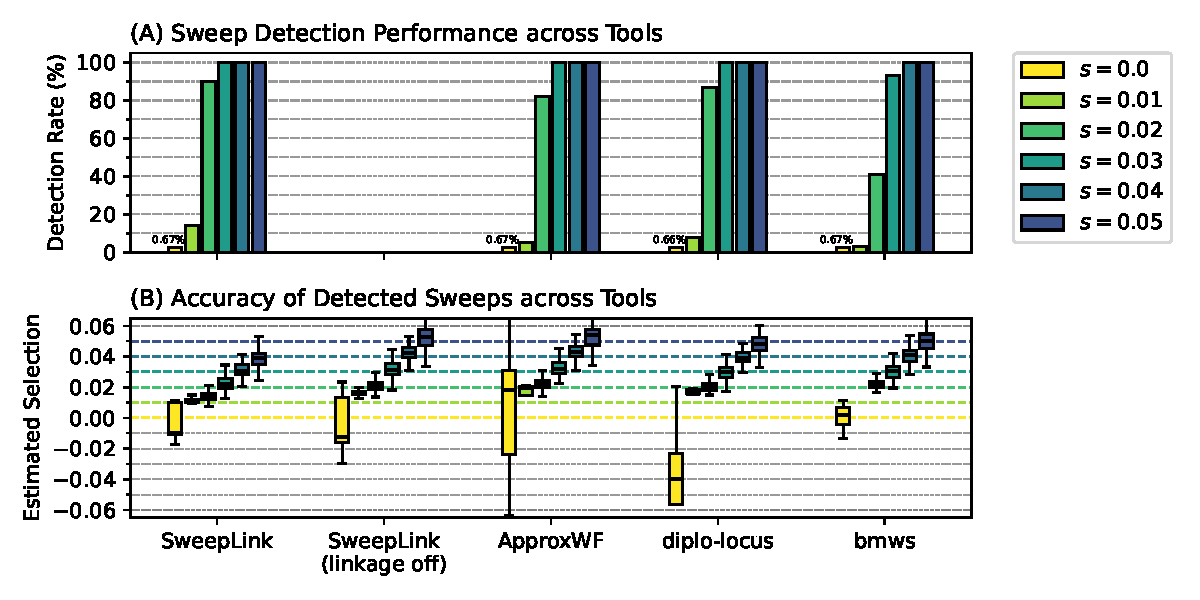
\includegraphics[width=0.8\textwidth]{figures/master_plots/comparison_master_plot_no1M_with_round2.pdf}
\caption{\textbf{Performance and estimation accuracy for selection detection tools.}
\textbf{(A)}~Sweep detection rates across selection coefficients evaluated at a matched window-based False Positive Rate (FPR) of 0.3\% (the empirical FPR of \SweepLink at $1-P \sim 10^{-5}$).
\SweepLink uniquely retains sensitivity for weak selection ($s=0.01$).
\textbf{(B)}~Estimated selection coefficients ($\hat{s}$) for loci passing the 0.3\% FPR threshold.
Coloured dashed lines indicate true values.
Most existing tools overestimate selection magnitude for false positives ($s=0.0$, yellow) and weak sweeps ($s=0.01$, light green).
In contrast, \SweepLink tightly constrains neutral errors near zero and provides highly accurate estimates for all selection coefficients, including weak selection ($s=0.01$).
}
\label{fig:results:tools_comparison}
\end{figure}

We then compared the accuracy of the estimated selection coefficients ($\hat{s}$) across tools (Figure~\ref{fig:results:tools_comparison}B).
To avoid biasing our distributions towards neutrality, we restricted this comparison strictly to loci predicted to be under selection, using the same thresholds defined previously (FPR=0.3\%).
Our results show that \diplolocus and \ApproxWF exhibit extreme variance when generating false positive calls---incorrectly predicting selection coefficients of high magnitude for strictly neutral sites ($s=0.0$).
This result is visualized by the yellow boxplots in Figure~\ref{fig:results:mcc_plot}B.
This behavior is expected, as these tools analyze each locus independently and only detect selection when random genetic drift happens to mimic a strong selective sweep.
While \ApproxWF shows more positive estimations for false positive calls, \diplolocus produce more high negative estimations.
We note that such estimations can be easily mixed with a true sweeps even for \diplolocus as sometimes polarization error may happen and then the sign of predicted selection will swap making it indistinguishable from the true sweep at $s=0.05$.
By leveraging regional genomic context, \SweepLink overcomes this limitation, yielding much more narrow confidence interval of estimations for trully neutral variants that is tightly constrained near zero.

When comparing estimates for selected variants, competitive methods routinely overestimate weak selective sweeps ($s=0.01$).
Similar to the high-magnitude estimates for neutral loci, this bias occurs because weak sweeps become significant only when random genetic drift happens to magnify the signal, producing a trajectory that mimics a much stronger sweep (e.g., $s \approx 0.02$).
In contrast, \SweepLink provided highly accurate and unbiased estimates for weak selection ($s=0.01$).
For actual stronger selective sweeps ($s \ge 0.02$), single-locus methods successfully and accurately estimated the true selection coefficients, with their median predictions closely tracking the simulated values.
The median estimates of \SweepLink scaled proportionally with the true selection strength, perfectly preserving the relative ranking of the effect sizes.
However, those predictions were systematically underestimated for all $s \ge 0.02$.
An inspection of the model's likelihood profiles reveals the mechanism driving this conservative bias.
Although the likelihood surface at the causal locus correctly peaks near the true value, it remains relatively flat around this maximum, a characteristic that becomes more pronounced at higher selection strengths.
Because the regional genomic model integrates data from linked passenger SNPs---which inherently experience progressively weaker apparent selection due to recombination---this flat likelihood space allows the surrounding context to computationally ``pull down'' the final joint estimate.

Crucially, further investigation revealed that the magnitude and direction of this bias depend heavily on the causal allele's frequency at the start of the sampling period (Figure~\ref*{fig:supp:performance:start_freq}).
The systematic underestimation observed previously is characteristic of our primary dataset's parameters, where sampling was initiated only after the causal variant's frequency exceeded $0.3$.
However, as this initial sampling frequency increases---which corresponds to capturing an older causal variant with a different genomic background---the selection estimates consistently shift upwards.
Consequently, when observing sweeps that are already at higher standing frequencies, the model overcomes its initial conservative bias and eventually begins to overestimate the selection coefficient.

To comprehensively evaluate the performance of \SweepLink's joint inference framework, we systematically assessed its accuracy and robustness across a diverse array of evolutionary scenarios and study designs.



\subsection{Validation on Simulated Data}
We evaluated how the accuracy of SweepLink inference depends on various experimental characteristics, including sample size, number of time points, sequence length, binning strategy, initial frequency of the selected allele, recombination rate, and the numerical grid size used for diffusion approximation.
To ensure a systematic comparison, we establish a default configuration for our simulations and then vary one characteristic at a time, keeping all other parameters fixed at their default values.

In each simulation, there are six simulated chromosomes  of the same length: three chromosomes containing only neutral variants, and three chromosomes, each with one causal variant under positive selection with selection coefficients of 0.01, 0.02, or 0.05.
For each experimental setup, simulation and subsequent inference were repeated 100 times.

For each value of the characteristic being varied, we report the power of \SweepLink to predict selection and the corresponding AUC scores.
Power is measured as the percentage of runs in which the posterior probability of selection for a variant exceeds 99\%.
We report AUC scores for each selection coefficient to provide a comprehensive measure that accounts for both true and false predictions of selection.
We also report the posterior distributions of the estimated selection coefficients and population size for each experiment.

In case of default configuration, SweepLink is able to detect selection in 40\% of cases for a selection coefficient of 0.01, in 96\% of cases for 0.02, and in 100\% of cases for 0.05.
On average, the method has a false positive rate of 2.3\%, meaning that it predicts selection for 2.3\% of neutral variants.
Generally, sweepLink has a tendency to underestimate selection coefficients and population size.
The lower estimation of population size is connected to high percentage (50\%) of data affected by selection.

The power to detect selection at causal variants, as well as AUC scores, increases with larger sample sizes.
SweepLink is unable to accurately estimate population size with small sample sizes (5 and 10 diploid individuals), but estimation improves substantially with larger samples, reaching the highest accuracy at 500 diploid samples per time point.
When estimating the selection coefficient on a grid, the posterior credible interval becomes narrower as the sample size increases.

A similar pattern is observed for the number of time points: both selection and population size inference accuracy with SweepLink improve as more time points are included.

Chromosome length does not affect the accuracy of selection inference, but longer sequences yield more concentrated posterior distributions for population size.
Notably, population size tends to be underestimated.
While estimation improves with increasing sequence length, the maximum length tested was insufficient to consistently recover the true population size.

SweepLink shows minimal sensitivity to binning.
The power to detect selection and resulting AUC scores remain relatively stable across bin sizes, with only small fluctuations.
However, confidence intervals for population size estimation increase with bin size.
For the largest binning tested (bin size 80, resulting in two bins and three time points), SweepLink consistently fails to estimate the correct population size.

The initial frequency of the derived allele strongly influences SweepLink’s power to detect selection.
Detection increases as derived allele frequency rises to 0.2–0.3, but power declines again at higher frequencies (0.8–0.9), producing a characteristic increase and decrease in detection power.
Meanwhile, mean population size estimates decrease as initial derived allele frequency increases, reflecting the prolonged action of selection and its effect on population size inference.

SweepLink leverages linkage information to improve selection inference, which is expected to be more effective under lower recombination rates.
As observed, selection inference improves as the recombination rate decreases from $10^{-5}$ to $10^{-8}$.
However, at an extremely low rate ($10^{-9}$) and short chromosome length (0.1 Mb), power to detect selection declines, likely due to excessive linkage.

Finally, increasing the resolution of the numerical grid in the Wright-Fisher diffusion scheme enhances SweepLink’s power to detect selection.
However, population size estimation remains inaccurate across all grid sizes tested, with the highest uncertainty observed at 100 grid points.
Importantly, selection is still inferred accurately, even when population size estimation is unreliable.

\subsection{Selection in British population}
We identified Y significant peaks of directed selection.
To understand the functional context of these signals, we mapped each focal SNP to nearby genes and assessed whether it overlaps with known regulatory elements, such as enhancers or promoters.
Furthermore to investigate the phenotypic targets of selection, we queried each focal SNP against UK Biobank GWAS summary statistics (Neale lab)~\citep{nealelab2018} via the OpenGWAS platform~\citep{elsworth2020}.
We then performed colocalization analysis between the predicted selection magnitudes and GWAS $p$-values within a 1 Mb window around each SNP.
Using this approach, we successfully identified a putative trait driving the selection signal for most of these regions (X out of Y peaks).
To explore the genomic architecture of these mapped regions, we examined their local selection profiles and GWAS association tracks alongside population-matched recombination map from the 1000 Genomes Project (GBR population) \citep{1000G2015}.
As illustrated in Figures~\ref{fig:X}-\ref{fig:Y}, this landscape analysis revealed a consistent pattern: the majority of our identified selection peaks are situated within recombination coldspots.
Additionally, the selection footprint inferred at the \textit{LCT} locus---a well-known target of selection for lactase persistence---aligns almost perfectly with the European LD block defined by LDetect \citep{berisa2015} (Figure~\ref{fig:results:brits_2chr_lct_region}).
\begin{figure}[tb]
\centering
    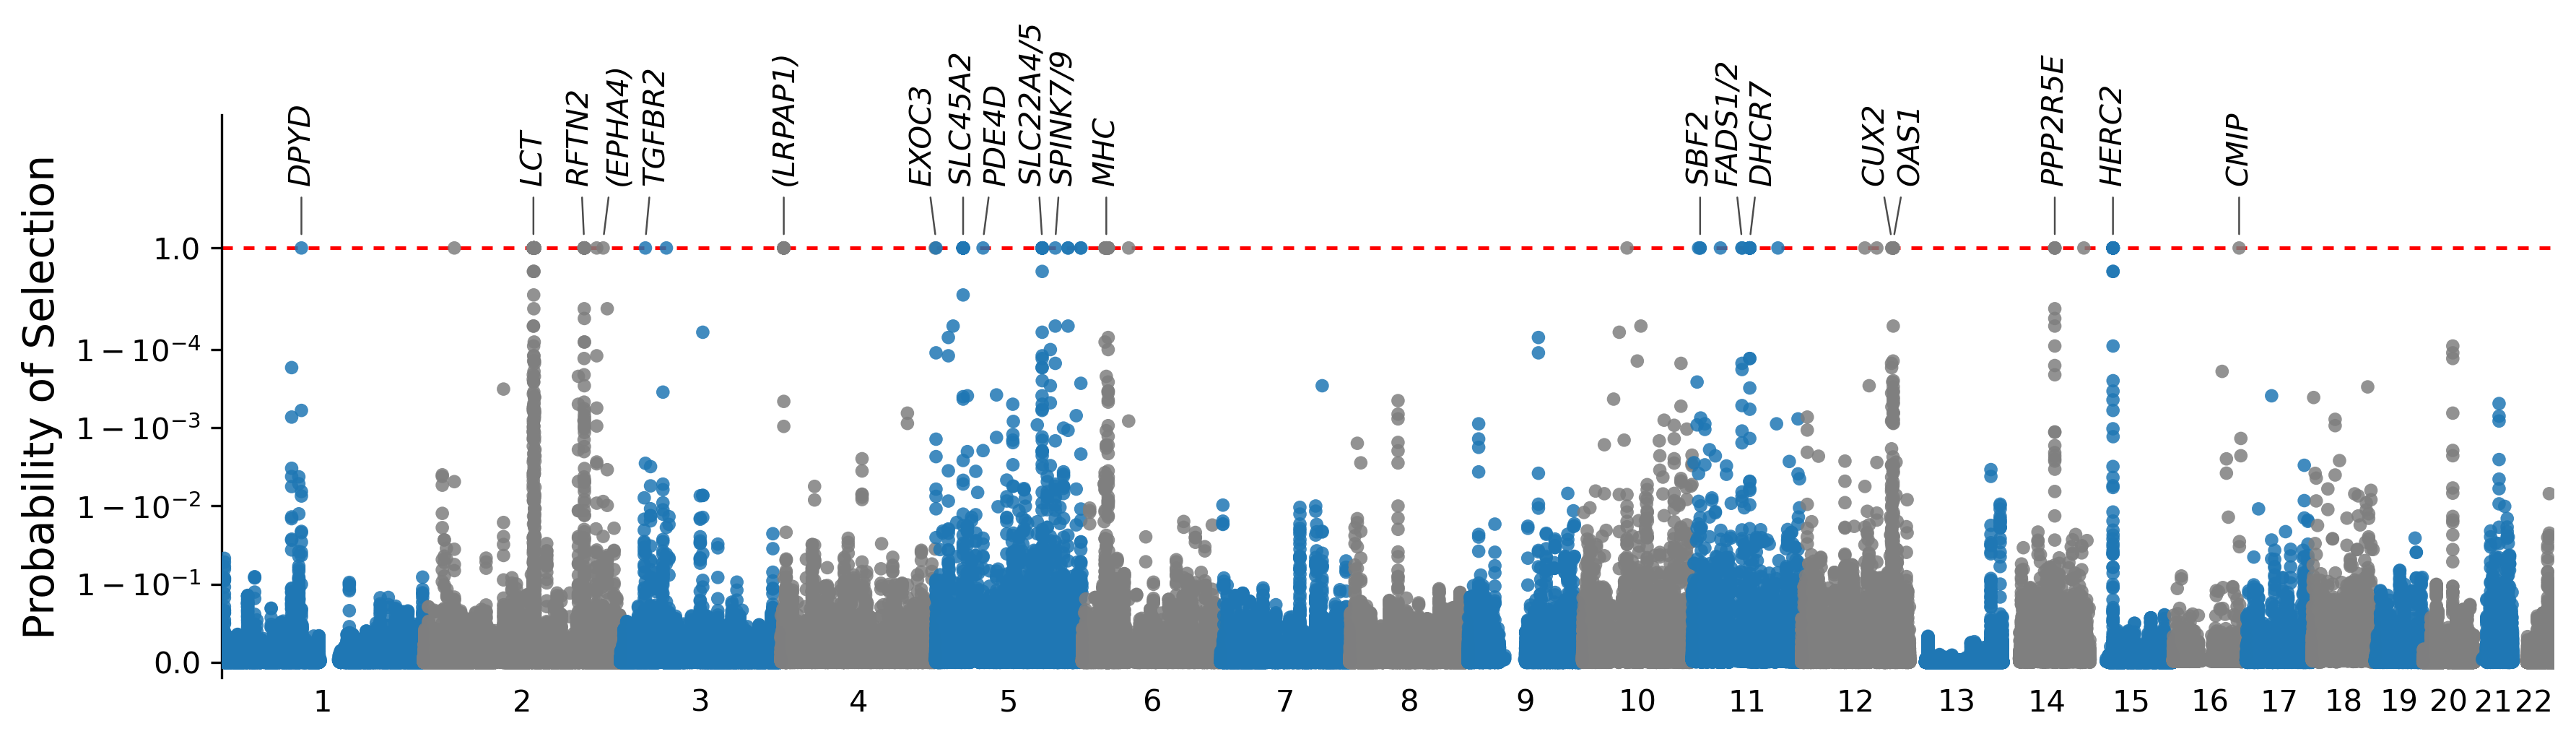
\includegraphics[width=\textwidth]{figures/real_data_results/manhattan_manuscript.png}
    \caption{
    \textbf{Genome-wide scan for signals of directed selection in Britain.}
    The y-axis reflects the posterior one-sided probability of selection ($P = \max(P(s>0), P(s<0))$), with the red dashed line representing the peak model confidence threshold ($P=1.0$).
    Top-scoring variants within notable genomic regions are annotated with their respective candidate genes.
    Five prominent peaks with intergenic variants (chromosome 4, 9, 10, 11 and 14) reaching the significance threshold remain unannotated due to a lack of identifiable candidate genes or established GWAS associations at those loci.
    }
    \label{fig:results:brits_manhattan_plot}
\end{figure}

\begin{figure}[tb]
\centering
    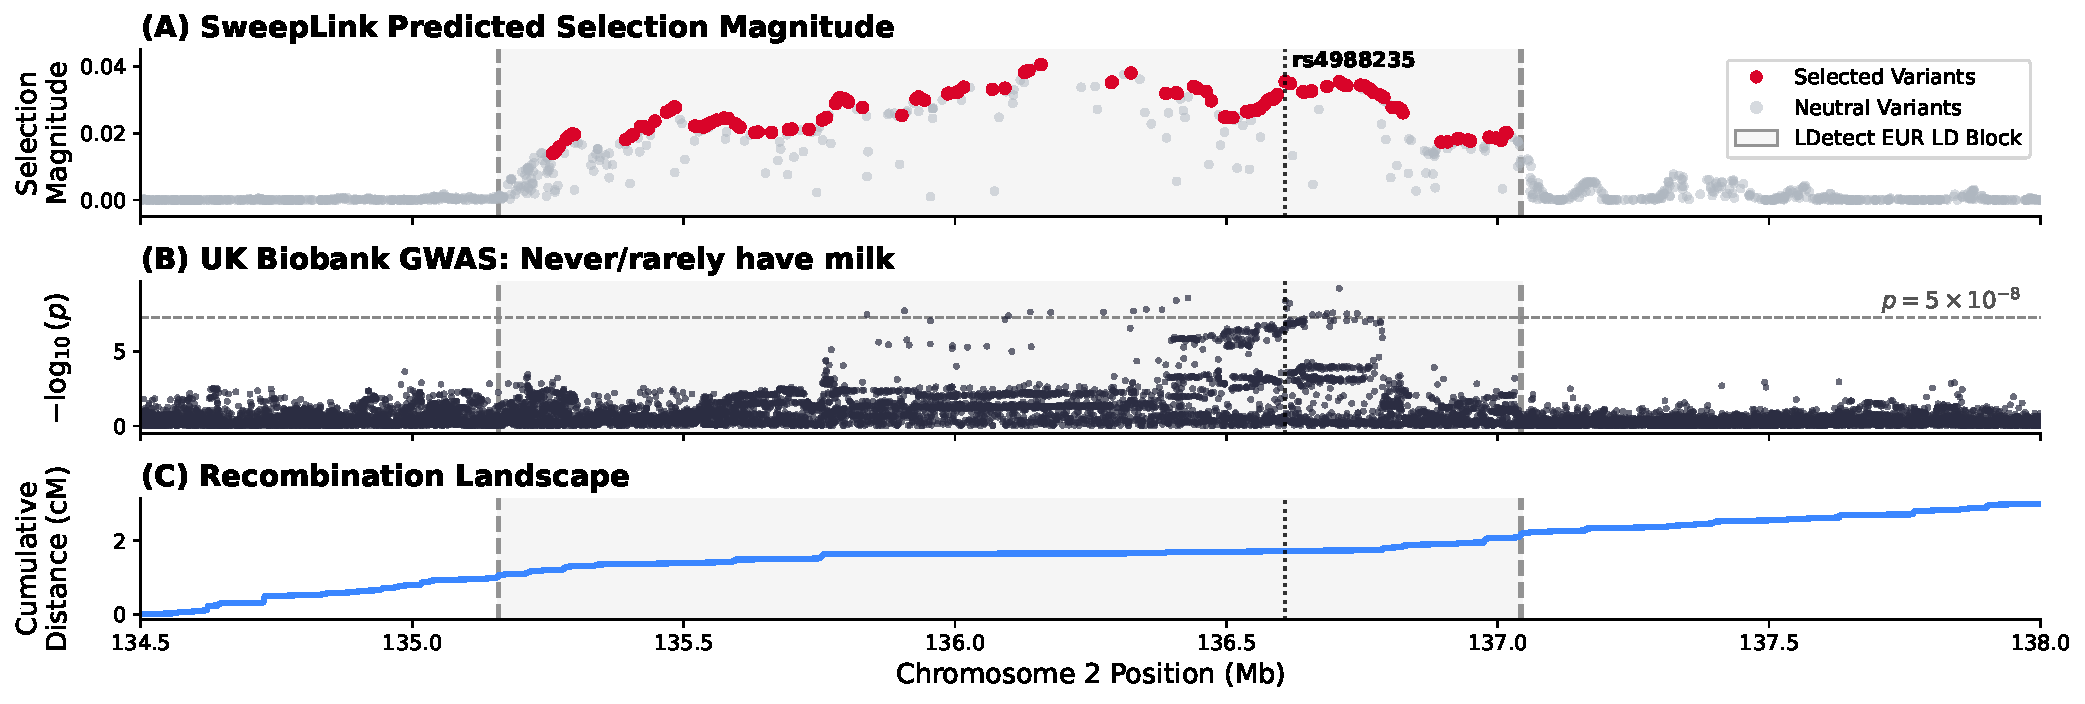
\includegraphics[width=\textwidth]{figures/real_data_results/region_plots/plot_sel_chr2_rs4988235.pdf}
    \caption{
    \textbf{Genomic landscape of the selection signal at the \textit{LCT} locus on chromosome 2.}
    (A) Predicted selection magnitudes generated by \SweepLink.
    Red points indicate variants classified as target variants under selection ($P=1.0$), while gray points represent neutral variants.
    The known causal variant for lactase persistence, rs4988235, is marked by a vertical dotted line.
    The shaded background bounded by dashed vertical lines represents the European linkage disequilibrium (LD) block derived from the LDetect database.
    (B) Local Manhattan plot of GWAS summary statistics from the UK Biobank (Neale lab) for the trait "Milk type used: Never/rarely have milk" (\mbox{OpenGWAS~ID:~ukb-d-1418\_6}).
    This trait colocalizes with predicted selection signal (colocalization probability = 0.99). The horizontal dashed line denotes the standard genome-wide significance threshold ($p=5 \times 10^{-8}$).
    (C) Cumulative recombination landscape (cM) based on the 1000 Genomes Project genetic map for the GBR population.
    }
    \label{fig:results:brits_2chr_lct_region}
\end{figure}

We compared the results of \SweepLink to a previous selection scan conducted on the same dataset \citep{mathieson2022}.
\SweepLink confirmed three of the seven primary regions previously reported to be under selection: \textit{LCT} (chromosome 2), \textit{DHCR7} (chromosome 22), and \textit{HERC2} (chromosome 15).
Conversely, our results do not support the previously predicted selection signal at the \textit{SLC45A2} locus on chromosome 5, yielding a minimum posterior probability of neutrality of 0.2 in this region.
Within the MHC region, \SweepLink detected a single peak localized to the \textit{HCP5B} gene, in contrast to the three distinct regions reported by \citet{mathieson2022}.
Additionally, \SweepLink showed no signs of selection in two regions on chromosomes 4 and 12 that were previously flagged as false positives \citep{mathieson2022}. % TODO: double check for chrom 12!
Overall, our scan identified X novel candidate regions under selection that were not detected in the previous analysis.


\begin{table}[htbp]
    \centering
    \caption{Regions under directed selection with colocalising trait associations.
    Selection coefficients ($\hat{s}$) refer to the derived allele, polarised against
    the Ensembl GRCh37 ancestral reconstruction; variants are written as
    ancestral\textgreater derived. ``Loci'' is the number of variants in the region
    at which all $10^5$ MCMC iterations agreed on the sign of $s$. Genes are the
    annotation at the region's position; parentheses mark a target variant lying
    outside the named gene. PP$_4$ is the posterior probability that the selection
    and trait signals share a causal variant.}
    \label{tab:selected_variants}
    \resizebox{\columnwidth}{!}{%
    \begin{tabular}{c r r l l r l r}
        \toprule
        & \multicolumn{5}{c}{\textbf{Selection}} & \multicolumn{2}{c}{\textbf{Colocalisation}} \\
        \cmidrule(lr){2-6} \cmidrule(lr){7-8}
        \textbf{Chr} & \textbf{Region (Mb)} & \textbf{Loci} & \textbf{Target variant} &
        \textbf{Gene} & \textbf{$\hat{s}$} & \textbf{Trait} & \textbf{PP$_4$} \\
        \midrule
        1  & $98.30$–$98.42$   & $1$   & rs12062845 C\textgreater A & DPYD          & $-0.0163$ & Waist circumference   & $0.98$ \\
        2  & $135.15$–$137.09$ & $177$ & rs4988235 G\textgreater A  & LCT/MCM6      & $+0.0313$ & Milk consumption      & $0.99$ \\
        2  & $198.14$–$198.97$ & $12$  & rs1455653 A\textgreater G  & RFTN2         & $-0.0157$ & Ankle spacing width   & $0.97$ \\
        5  & $0.42$–$0.46$     & $1$   & rs2251843 G\textgreater A  & EXOC3         & $+0.0109$ & Haematocrit           & $0.99$ \\
        5  & $33.88$–$34.00$   & $14$  & rs16891982 C\textgreater G & SLC45A2       & $+0.0299$ & Skin colour           & $0.99$ \\
        5  & $131.53$–$131.72$ & $11$  & rs273901 T\textgreater G$^\ddagger$ & SLC22A4/5 & $-0.0149$ & \textit{SLC22A4/5} expression & $0.99$ \\
        5  & $147.68$–$147.76$ & $1$   & rs1363707 A\textgreater G  & SPINK7/9      & $-0.0141$ & Pulse pressure        & $0.98$ \\
        6  & $28.21$–$28.36$   & $3$   & rs6912584 T\textgreater C  & (ZKSCAN3/ZSCAN31) & $+0.0221$ & Coeliac disease   & $0.96$ \\
        6  & $29.82$–$29.89$   & $7$   & rs3132714 T\textgreater C$^\dagger$ & HLA-F/HLA-G & $+0.0177$ & Haemoglobin conc. & $0.89$ \\
        6  & $32.03$–$32.18$   & $5$   & rs204994 C\textgreater T   & (AGER/PBX2)   & $+0.0257$ & Bioavailable testosterone & $1.00$ \\
        11 & $61.55$–$61.62$   & $2$   & rs174547 C\textgreater T   & FADS1/FADS2   & $+0.0139$ & Cholesterol           & $0.99$ \\
        11 & $71.12$–$71.22$   & $14$  & rs12800438 A\textgreater G & NADSYN1/DHCR7 & $-0.0243$ & Vitamin D             & $0.99$ \\
        12 & $111.24$–$111.69$ & $2$   & rs1034603 A\textgreater G  & CUX2          & $-0.0151$ & Platelet crit         & $0.99$ \\
        12 & $113.32$–$113.38$ & $5$   & rs4767028 A\textgreater G  & OAS1          & $-0.0148$ & OAS1 protein levels   & $0.99$ \\
        14 & $63.78$–$63.88$   & $4$   & rs28409133 T\textgreater G & (PPP2R5E)     & $-0.0301$ & Standing height       & $0.92$ \\
        15 & $28.31$–$28.54$   & $12$  & rs12913832 A\textgreater G & HERC2         & $+0.0227$ & Skin colour           & $0.94$ \\
        \bottomrule
    \end{tabular}%
    }
    \\[2pt]
    \footnotesize $^{\dagger}$No ancestral allele call at rs3132714 (Ensembl reports \texttt{AA=N}); sign of selection is relative to the alternate allele.
    $^{\ddagger}$Low-confidence ancestral call at rs273901 (Ensembl reports \texttt{AA=t}).
\end{table}

\begin{table}[t]
\centering\footnotesize
\setlength{\tabcolsep}{3pt}
\caption{Regions under selection without independent functional support.
\emph{Tested} indicates colocalisation was run against every trait associated
with the lead variant and no shared causal variant was recovered;
\emph{no coloc.}\ that no association reached genome-wide significance to test.
\emph{Corr., no LD} marks regions whose neighbouring loci show correlated
allele-frequency trajectories while carrying no linkage disequilibrium, which
\textsc{SweepLink} cannot distinguish from a sweep because its input carries no
haplotype information. $n$ is the number of variants in the region.}
\label{tab:unsupported}
\begin{tabular}{@{}clrlcl>{\raggedright\arraybackslash}p{2.3cm}@{}}
\toprule
Chr & Region (Mb) & $n$ & Lead SNP & $s$ & Freq & Status \\
\midrule
2  & 37.94--38.01   & 50 & rs72791933  & $-0.0099$ & $0.32\!\to\!0.00$ & Corr., no LD \\
2  & 213.76--213.82 & 36 & rs10498001  & $+0.0141$ & $0.12\!\to\!0.20$ & Tested, PP4 0.00 \\
2  & 221.74--221.79 & 18 & rs830747    & $-0.0126$ & $0.22\!\to\!0.76$ & No coloc. \\
3  & 30.71--30.73   & 21 & rs3773656   & $+0.0143$ & $0.75\!\to\!0.04$ & No coloc. \\
3  & 56.62--56.67   & 16 & rs282534    & $+0.0195$ & $0.42\!\to\!0.91$ & Tested, PP4 0.00 \\
4  & 190.64--190.69 & 5  & rs11132751  & $-0.0254$ & $0.74\!\to\!0.03$ & No coloc. \\
5  & 58.50--58.55   & 25 & rs66803649  & $+0.0164$ & $0.33\!\to\!0.99$ & No GWAS association \\
5  & 163.50--163.53 & 10 & rs10462943  & $+0.0165$ & $0.29\!\to\!0.56$ & Corrupted $p$-values \\
5  & 179.22--179.37 & 45 & rs27471     & $+0.0141$ & $0.57\!\to\!0.71$ & No coloc. \\
6  & 57.45--57.47   & 3  & rs9396343$^{*}$ & $+0.0253$ & $0.35\!\to\!0.78$ & No GWAS association \\
10 & 55.10--55.15   & 20 & rs10825008  & $+0.0171$ & $0.46\!\to\!0.71$ & No coloc. \\
11 & 7.96--7.98     & 17 & rs907203    & $+0.0159$ & $0.05\!\to\!0.51$ & Corr., no LD \\
11 & 9.84--9.88     & 17 & rs2403221   & $+0.0201$ & $0.44\!\to\!0.79$ & Tested, PP4 0.29 \\
11 & 34.94--34.95   & 26 & rs2956103   & $-0.0105$ & $0.71\!\to\!0.21$ & No coloc. \\
11 & 105.93--105.95 & 3  & rs10895900  & $+0.0234$ & $0.20\!\to\!0.75$ & No coloc. \\
12 & 78.30--78.35   & 20 & rs17817928  & $-0.0116$ & $0.29\!\to\!0.10$ & Corr., no LD \\
12 & 93.06--93.10   & 14 & rs937754    & $-0.0131$ & $0.70\!\to\!0.92$ & No coloc. \\
14 & 99.75--99.76   & 8  & rs5013941   & $+0.0159$ & $0.73\!\to\!0.08$ & No coloc. \\
16 & 81.62          & 1  & rs4503787   & $+0.0336$ & $0.06\!\to\!0.58$ & Tested, PP4 0.50 \\
\bottomrule
\end{tabular}
\\[2pt]
\footnotesize $^{*}$Low-confidence ancestral call at rs9396343 (Ensembl reports \texttt{AA=c}); the magnitude of $s$ is unaffected, the sign is not.
\end{table}

\section{Discussion}

\SweepLink is the first tool for the joint estimate of demography and linked selection from genome-wide time-series data.
Correlations between nearby loci, that \SweepLink captures, allows it to pull evidence of selection to improve detection power for weak selection compared to other existing single-locus methods.
At the same time isolated loci that happen to mimic selection sweep due to genetic drift are pushed to neutrality as they are not supported by their background.

Our experiments demonstrated that \SweepLink is more sensitive to weak and moderate selection than other tools, while its detection power for strong selection is the same.
When sweeplink is able to capture the correlation between loci then it produce highly polarized posteriors, that lead to best performance on the high stringency.
Compared to other existing methods this provides an advantage on practice: while other tool require an empirical threshold to separate neutral loci from selected and highly depend on this choice, \SweepLink provides best estimates on its highest stringency level.
This eliminates the dependency on the threshold.
When \SweepLink fails to estimate the correlation structure along the genome, then it converges to the behaviour of single-loci tools.

Our experiments on simulated data 

% our best filtering kind of make sense because our model does not account for allele to be lost


\bibliography{sample}

\end{document}